\documentclass[twoside]{book}

% Packages required by doxygen
\usepackage{fixltx2e}
\usepackage{calc}
\usepackage{doxygen}
\usepackage[export]{adjustbox} % also loads graphicx
\usepackage{graphicx}
\usepackage[utf8]{inputenc}
\usepackage{makeidx}
\usepackage{multicol}
\usepackage{multirow}
\PassOptionsToPackage{warn}{textcomp}
\usepackage{textcomp}
\usepackage[nointegrals]{wasysym}
\usepackage[table]{xcolor}

% Font selection
\usepackage[T1]{fontenc}
\usepackage[scaled=.90]{helvet}
\usepackage{courier}
\usepackage{amssymb}
\usepackage{sectsty}
\renewcommand{\familydefault}{\sfdefault}
\allsectionsfont{%
  \fontseries{bc}\selectfont%
  \color{darkgray}%
}
\renewcommand{\DoxyLabelFont}{%
  \fontseries{bc}\selectfont%
  \color{darkgray}%
}
\newcommand{\+}{\discretionary{\mbox{\scriptsize$\hookleftarrow$}}{}{}}

% Page & text layout
\usepackage{geometry}
\geometry{%
  a4paper,%
  top=2.5cm,%
  bottom=2.5cm,%
  left=2.5cm,%
  right=2.5cm%
}
\tolerance=750
\hfuzz=15pt
\hbadness=750
\setlength{\emergencystretch}{15pt}
\setlength{\parindent}{0cm}
\setlength{\parskip}{3ex plus 2ex minus 2ex}
\makeatletter
\renewcommand{\paragraph}{%
  \@startsection{paragraph}{4}{0ex}{-1.0ex}{1.0ex}{%
    \normalfont\normalsize\bfseries\SS@parafont%
  }%
}
\renewcommand{\subparagraph}{%
  \@startsection{subparagraph}{5}{0ex}{-1.0ex}{1.0ex}{%
    \normalfont\normalsize\bfseries\SS@subparafont%
  }%
}
\makeatother

% Headers & footers
\usepackage{fancyhdr}
\pagestyle{fancyplain}
\fancyhead[LE]{\fancyplain{}{\bfseries\thepage}}
\fancyhead[CE]{\fancyplain{}{}}
\fancyhead[RE]{\fancyplain{}{\bfseries\leftmark}}
\fancyhead[LO]{\fancyplain{}{\bfseries\rightmark}}
\fancyhead[CO]{\fancyplain{}{}}
\fancyhead[RO]{\fancyplain{}{\bfseries\thepage}}
\fancyfoot[LE]{\fancyplain{}{}}
\fancyfoot[CE]{\fancyplain{}{}}
\fancyfoot[RE]{\fancyplain{}{\bfseries\scriptsize Generated by Doxygen }}
\fancyfoot[LO]{\fancyplain{}{\bfseries\scriptsize Generated by Doxygen }}
\fancyfoot[CO]{\fancyplain{}{}}
\fancyfoot[RO]{\fancyplain{}{}}
\renewcommand{\footrulewidth}{0.4pt}
\renewcommand{\chaptermark}[1]{%
  \markboth{#1}{}%
}
\renewcommand{\sectionmark}[1]{%
  \markright{\thesection\ #1}%
}

% Indices & bibliography
\usepackage{natbib}
\usepackage[titles]{tocloft}
\setcounter{tocdepth}{3}
\setcounter{secnumdepth}{5}
\makeindex

% Hyperlinks (required, but should be loaded last)
\usepackage{ifpdf}
\ifpdf
  \usepackage[pdftex,pagebackref=true]{hyperref}
\else
  \usepackage[ps2pdf,pagebackref=true]{hyperref}
\fi
\hypersetup{%
  colorlinks=true,%
  linkcolor=blue,%
  citecolor=blue,%
  unicode%
}

% Custom commands
\newcommand{\clearemptydoublepage}{%
  \newpage{\pagestyle{empty}\cleardoublepage}%
}

\usepackage{caption}
\captionsetup{labelsep=space,justification=centering,font={bf},singlelinecheck=off,skip=4pt,position=top}

%===== C O N T E N T S =====

\begin{document}

% Titlepage & ToC
\hypersetup{pageanchor=false,
             bookmarksnumbered=true,
             pdfencoding=unicode
            }
\pagenumbering{alph}
\begin{titlepage}
\vspace*{7cm}
\begin{center}%
{\Large C Extensions }\\
\vspace*{1cm}
{\large Generated by Doxygen 1.8.13}\\
\end{center}
\end{titlepage}
\clearemptydoublepage
\pagenumbering{roman}
\tableofcontents
\clearemptydoublepage
\pagenumbering{arabic}
\hypersetup{pageanchor=true}

%--- Begin generated contents ---
\chapter{Overview}
\label{index}\hypertarget{index}{}C Extensions, or CX for short, is a collection of extensions to the C programing language, packaged as a single shared library. These extensions include exception handling, automatic dynamic memory deallocation and destruction, a universal object interface, and generic containers. The library is written in C and is not hardware dependent. Currently only P\+O\+S\+IX platforms are supported but a Windows port is planned. Please note that this project is still in the early stages of development. 
\chapter{C Extensions}
\label{a00083}
\Hypertarget{a00083}
\section*{C Extensions}

\subsubsection*{Overview}

C Extensions, or CX for short, is a collection of extensions to the C programing language, packaged as a single shared library. These extensions include exception handling, automatic dynamic memory deallocation and destruction, a universal object interface, and generic containers. The library is written in C and is not hardware dependent. Currently only P\+O\+S\+IX platforms are supported but a Windows port is planned. Please note that this project is still in the early stages of development. \subsubsection*{Documentation}

\href{https://codrod.github.io/cx/index.html}{\tt https\+://codrod.\+github.\+io/cx/index.\+html} \subsubsection*{Build Instructions}


\begin{DoxyItemize}
\item make 
\item make examples 
\item make test 
\item make docs 
\end{DoxyItemize}

Running \textquotesingle{}make test\textquotesingle{} will generate a script \textquotesingle{}test.\+sh\textquotesingle{} which is used to start the automated unit testing. 

\subsubsection*{Status}


\begin{DoxyItemize}
\item exception handling -\/ completed 
\item memory management -\/ completed 
\item strings -\/ completed 
\item universal object interface -\/ in progress 
\item generic containers -\/ not started 
\end{DoxyItemize}\subsubsection*{Development Plan}


\begin{DoxyEnumerate}
\item Complete current features 
\item Improve documentation 
\item Optimize 
\item Windows port 
\end{DoxyEnumerate}
\chapter{Class Index}
\section{Class List}
Here are the classes, structs, unions and interfaces with brief descriptions\+:\begin{DoxyCompactList}
\item\contentsline{section}{\hyperlink{structcxexception}{cxexception} }{\pageref{structcxexception}}{}
\item\contentsline{section}{\hyperlink{structcxmem__storage}{cxmem\+\_\+storage} }{\pageref{structcxmem__storage}}{}
\item\contentsline{section}{\hyperlink{structcxstring}{cxstring} }{\pageref{structcxstring}}{}
\item\contentsline{section}{\hyperlink{structcxui}{cxui} }{\pageref{structcxui}}{}
\end{DoxyCompactList}

\chapter{File Index}
\section{File List}
Here is a list of all documented files with brief descriptions\+:\begin{DoxyCompactList}
\item\contentsline{section}{include/\hyperlink{cxdef_8h}{cxdef.\+h} \\*Contains defs for basic types used by the entire library }{\pageref{cxdef_8h}}{}
\item\contentsline{section}{include/\hyperlink{cxerror_8h}{cxerror.\+h} \\*Error codes shared by the entire library are defined here }{\pageref{cxerror_8h}}{}
\item\contentsline{section}{include/\hyperlink{cxex_8h}{cxex.\+h} \\*Exception handling }{\pageref{cxex_8h}}{}
\item\contentsline{section}{include/\hyperlink{cxlib_8h}{cxlib.\+h} \\*Single header file for entire library }{\pageref{cxlib_8h}}{}
\item\contentsline{section}{include/\hyperlink{cxmem_8h}{cxmem.\+h} \\*Memory management }{\pageref{cxmem_8h}}{}
\item\contentsline{section}{include/{\bfseries cxrt.\+h} }{\pageref{cxrt_8h}}{}
\item\contentsline{section}{include/{\bfseries cxrt\+\_\+mutex.\+h} }{\pageref{cxrt__mutex_8h}}{}
\item\contentsline{section}{include/\hyperlink{cxstring_8h}{cxstring.\+h} \\*Strings }{\pageref{cxstring_8h}}{}
\item\contentsline{section}{include/{\bfseries cxui.\+h} }{\pageref{cxui_8h}}{}
\end{DoxyCompactList}

\chapter{Class Documentation}
\hypertarget{a00048}{}\section{cxexception Struct Reference}
\label{a00048}\index{cxexception@{cxexception}}
\subsection*{Public Attributes}
\begin{DoxyCompactItemize}
\item 
\mbox{\Hypertarget{a00048_a21a3264050c2a040698bc6f37487c633}\label{a00048_a21a3264050c2a040698bc6f37487c633}} 
char $\ast$ {\bfseries type}
\item 
\mbox{\Hypertarget{a00048_a81aa35ab48089d35437efb5351ec2243}\label{a00048_a81aa35ab48089d35437efb5351ec2243}} 
char $\ast$ {\bfseries what}
\item 
\mbox{\Hypertarget{a00048_a58947b8f85613c5c0db0a78adc2035d1}\label{a00048_a58947b8f85613c5c0db0a78adc2035d1}} 
int {\bfseries ret}
\end{DoxyCompactItemize}


The documentation for this struct was generated from the following file\+:\begin{DoxyCompactItemize}
\item 
\hyperlink{a00011}{cxex.\+h}\end{DoxyCompactItemize}

\hypertarget{a00056}{}\section{cxmem\+\_\+storage Struct Reference}
\label{a00056}\index{cxmem\+\_\+storage@{cxmem\+\_\+storage}}


Collaboration diagram for cxmem\+\_\+storage\+:
\nopagebreak
\begin{figure}[H]
\begin{center}
\leavevmode
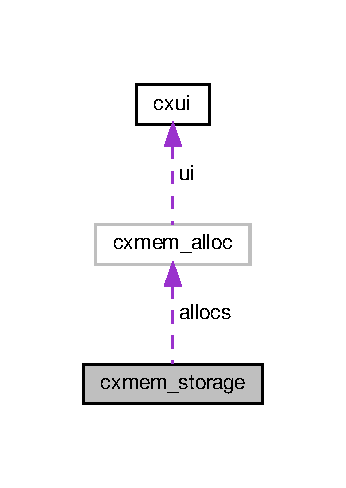
\includegraphics[width=166pt]{a00054}
\end{center}
\end{figure}
\subsection*{Public Attributes}
\begin{DoxyCompactItemize}
\item 
\mbox{\Hypertarget{a00056_a4663e63ea74aef2a831c26f29cec7147}\label{a00056_a4663e63ea74aef2a831c26f29cec7147}} 
cxmem\+\_\+alloc\+\_\+t $\ast$ {\bfseries allocs}
\item 
\mbox{\Hypertarget{a00056_ae0e190eb4581da409bcf0c1709852e9f}\label{a00056_ae0e190eb4581da409bcf0c1709852e9f}} 
cxsize\+\_\+t {\bfseries size}
\item 
\mbox{\Hypertarget{a00056_a631394e8755be3e93cd90beeeb51ff3c}\label{a00056_a631394e8755be3e93cd90beeeb51ff3c}} 
cxsize\+\_\+t {\bfseries cap}
\item 
\mbox{\Hypertarget{a00056_a9c77308d0cf6fc2016ebaaafc77e0402}\label{a00056_a9c77308d0cf6fc2016ebaaafc77e0402}} 
cxrt\+\_\+mutex\+\_\+t $\ast$ {\bfseries mutex}
\end{DoxyCompactItemize}


The documentation for this struct was generated from the following file\+:\begin{DoxyCompactItemize}
\item 
\hyperlink{a00017}{cxmem.\+h}\end{DoxyCompactItemize}

\hypertarget{a00072}{}\section{cxstring Struct Reference}
\label{a00072}\index{cxstring@{cxstring}}
\subsection*{Public Attributes}
\begin{DoxyCompactItemize}
\item 
\mbox{\Hypertarget{a00072_adbb4c5b19ff3e49e2da0776d1102da02}\label{a00072_adbb4c5b19ff3e49e2da0776d1102da02}} 
char $\ast$ {\bfseries data}
\item 
\mbox{\Hypertarget{a00072_a8ee64de5ade5635f6609c8fd26a3d7ee}\label{a00072_a8ee64de5ade5635f6609c8fd26a3d7ee}} 
cxsize\+\_\+t {\bfseries index}
\item 
\mbox{\Hypertarget{a00072_a98ef2ad0212a946095e90ed9fe16a2d6}\label{a00072_a98ef2ad0212a946095e90ed9fe16a2d6}} 
cxsize\+\_\+t {\bfseries size}
\item 
\mbox{\Hypertarget{a00072_a38495c5af12925f89ad3a57c06d8fabe}\label{a00072_a38495c5af12925f89ad3a57c06d8fabe}} 
cxsize\+\_\+t {\bfseries cap}
\end{DoxyCompactItemize}


The documentation for this struct was generated from the following file\+:\begin{DoxyCompactItemize}
\item 
\hyperlink{a00026}{cxstring.\+h}\end{DoxyCompactItemize}

\hypertarget{a00076}{}\section{cxui Struct Reference}
\label{a00076}\index{cxui@{cxui}}
\subsection*{Public Attributes}
\begin{DoxyCompactItemize}
\item 
\mbox{\Hypertarget{a00076_a9edf2234d6c5e377b374b7d6c950bbf5}\label{a00076_a9edf2234d6c5e377b374b7d6c950bbf5}} 
char $\ast$ {\bfseries name}
\item 
\mbox{\Hypertarget{a00076_a51857dc6e083abb11aea3dfbd8cbcefe}\label{a00076_a51857dc6e083abb11aea3dfbd8cbcefe}} 
cxsize\+\_\+t {\bfseries size\+\_\+of}
\item 
\mbox{\Hypertarget{a00076_a875809f41c644cb1541c1432ca937ee7}\label{a00076_a875809f41c644cb1541c1432ca937ee7}} 
void($\ast$ {\bfseries construct} )(cxsize\+\_\+t size\+\_\+of, cxaddress\+\_\+t obj, va\+\_\+list $\ast$argv)
\item 
\mbox{\Hypertarget{a00076_a3d7dd83e42ba2a7d6a0aa49527162b90}\label{a00076_a3d7dd83e42ba2a7d6a0aa49527162b90}} 
void($\ast$ {\bfseries destruct} )(cxaddress\+\_\+t obj)
\item 
\mbox{\Hypertarget{a00076_a4c667e63ed3718837c8d72a61f08c5e7}\label{a00076_a4c667e63ed3718837c8d72a61f08c5e7}} 
int($\ast$ {\bfseries compare} )(cxsize\+\_\+t size\+\_\+of, const cxaddress\+\_\+t obj1, const cxaddress\+\_\+t obj2, va\+\_\+list $\ast$argv)
\item 
\mbox{\Hypertarget{a00076_abb0c082998801b196b4628c677d52355}\label{a00076_abb0c082998801b196b4628c677d52355}} 
int($\ast$ {\bfseries copy} )(cxsize\+\_\+t size\+\_\+of, cxaddress\+\_\+t des, const cxaddress\+\_\+t src)
\item 
\mbox{\Hypertarget{a00076_a0557283698a935aaa7975cfe7f988991}\label{a00076_a0557283698a935aaa7975cfe7f988991}} 
cxsize\+\_\+t($\ast$ {\bfseries string\+\_\+to} )(cxsize\+\_\+t size\+\_\+of, cxaddress\+\_\+t str, cxaddress\+\_\+t obj, va\+\_\+list $\ast$argv)
\item 
\mbox{\Hypertarget{a00076_a74e72113821a16a7c2e5d73c9a954d1e}\label{a00076_a74e72113821a16a7c2e5d73c9a954d1e}} 
cxsize\+\_\+t($\ast$ {\bfseries to\+\_\+string} )(cxsize\+\_\+t size\+\_\+of, const cxaddress\+\_\+t obj, cxaddress\+\_\+t str, va\+\_\+list $\ast$argv)
\end{DoxyCompactItemize}


The documentation for this struct was generated from the following file\+:\begin{DoxyCompactItemize}
\item 
cxui.\+h\end{DoxyCompactItemize}

\chapter{File Documentation}
\hypertarget{a00005}{}\section{cxdef.\+h File Reference}
\label{a00005}\index{cxdef.\+h@{cxdef.\+h}}


Contains defs for basic types used by the entire library.  


{\ttfamily \#include $<$stddef.\+h$>$}\newline
{\ttfamily \#include $<$stdint.\+h$>$}\newline
{\ttfamily \#include $<$limits.\+h$>$}\newline
Include dependency graph for cxdef.\+h\+:

\hypertarget{a00008}{}\section{cxerror.\+h File Reference}
\label{a00008}\index{cxerror.\+h@{cxerror.\+h}}


Error codes shared by the entire library are defined here.  


This graph shows which files directly or indirectly include this file\+:
\nopagebreak
\begin{figure}[H]
\begin{center}
\leavevmode
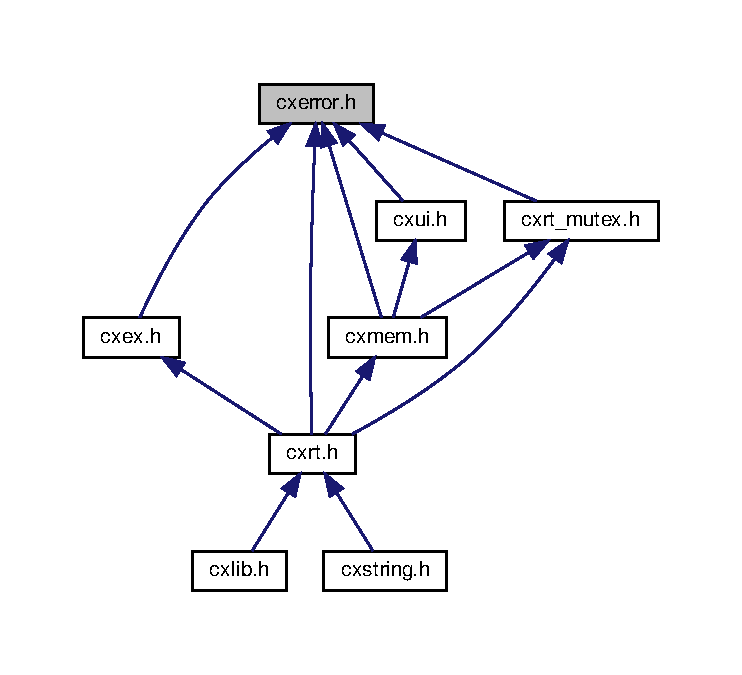
\includegraphics[width=350pt]{a00010}
\end{center}
\end{figure}
\subsection*{Macros}
\begin{DoxyCompactItemize}
\item 
\mbox{\Hypertarget{a00008_a5b8d52f060c8908fb025bd16201fbf49}\label{a00008_a5b8d52f060c8908fb025bd16201fbf49}} 
\#define {\bfseries C\+X\+E\+R\+R\+O\+R\+\_\+\+V\+E\+R\+S\+I\+ON}~1000000L
\item 
\mbox{\Hypertarget{a00008_ab600a2597512889da741a03cab3797e8}\label{a00008_ab600a2597512889da741a03cab3797e8}} 
\#define {\bfseries C\+X\+E\+R\+R\+O\+R\+\_\+\+M\+A\+IN}~-\/2018
\item 
\mbox{\Hypertarget{a00008_ad036caf4caff7b0dc9d41887337646f2}\label{a00008_ad036caf4caff7b0dc9d41887337646f2}} 
\#define {\bfseries C\+X\+E\+R\+R\+O\+R\+\_\+\+F\+U\+NC}~-\/2019
\item 
\mbox{\Hypertarget{a00008_a35bddeba7e57335e72010a3bfd324a71}\label{a00008_a35bddeba7e57335e72010a3bfd324a71}} 
\#define {\bfseries C\+X\+E\+R\+R\+O\+R\+\_\+\+T\+H\+R\+E\+AD}~-\/2020
\item 
\mbox{\Hypertarget{a00008_ae6621b332130a649e1e1684b3e1082f3}\label{a00008_ae6621b332130a649e1e1684b3e1082f3}} 
\#define {\bfseries C\+X\+E\+R\+R\+O\+R\+\_\+\+R\+E\+T\+U\+RN}~-\/2021
\item 
\mbox{\Hypertarget{a00008_a1ec6bc7be0b7c5985f97540d00c84de2}\label{a00008_a1ec6bc7be0b7c5985f97540d00c84de2}} 
\#define {\bfseries C\+X\+E\+R\+R\+O\+R\+\_\+\+T\+H\+R\+OW}~-\/2022
\item 
\mbox{\Hypertarget{a00008_a67aba3619760b88b100127a53a41cc16}\label{a00008_a67aba3619760b88b100127a53a41cc16}} 
\#define {\bfseries C\+X\+E\+R\+R\+O\+R\+\_\+\+T\+RY}~-\/2023
\item 
\mbox{\Hypertarget{a00008_a3c7905fc6441e714dbf9c9ad464a59c7}\label{a00008_a3c7905fc6441e714dbf9c9ad464a59c7}} 
\#define {\bfseries C\+X\+E\+R\+R\+O\+R\+\_\+\+N\+O\+M\+EM}~-\/2023
\item 
\mbox{\Hypertarget{a00008_ad20217630427985309eaaa7e5db79af6}\label{a00008_ad20217630427985309eaaa7e5db79af6}} 
\#define {\bfseries C\+X\+E\+R\+R\+O\+R\+\_\+\+E\+M\+P\+TY}~-\/2024
\item 
\mbox{\Hypertarget{a00008_a4ccd3f7805126c885e383fb35abf57f6}\label{a00008_a4ccd3f7805126c885e383fb35abf57f6}} 
\#define {\bfseries C\+X\+E\+R\+R\+O\+R\+\_\+\+A\+RG}~-\/2025
\item 
\mbox{\Hypertarget{a00008_a19b6c0e8af74f2867b458cf68be6eb23}\label{a00008_a19b6c0e8af74f2867b458cf68be6eb23}} 
\#define {\bfseries C\+X\+E\+R\+R\+O\+R\+\_\+\+S\+I\+G\+N\+AL}~-\/2026
\item 
\mbox{\Hypertarget{a00008_a658279061a52324f85003fd97afb154c}\label{a00008_a658279061a52324f85003fd97afb154c}} 
\#define {\bfseries C\+X\+E\+R\+R\+O\+R\+\_\+\+N\+O\+T\+\_\+\+F\+O\+U\+ND}~-\/2027
\item 
\mbox{\Hypertarget{a00008_a49e8e2410fe21c65f3bc858087f514f3}\label{a00008_a49e8e2410fe21c65f3bc858087f514f3}} 
\#define {\bfseries C\+X\+E\+R\+R\+O\+R\+\_\+\+A\+D\+D\+R\+E\+SS}~-\/2028
\item 
\mbox{\Hypertarget{a00008_a7512de878ea8479d3dd2f9c1efe35861}\label{a00008_a7512de878ea8479d3dd2f9c1efe35861}} 
\#define {\bfseries C\+X\+E\+R\+R\+O\+R\+\_\+\+S\+I\+ZE}~-\/2029
\item 
\mbox{\Hypertarget{a00008_a5d322d3ae6c6f0308125734673619399}\label{a00008_a5d322d3ae6c6f0308125734673619399}} 
\#define {\bfseries C\+X\+E\+R\+R\+O\+R\+\_\+\+P\+U\+SH}~-\/2030
\end{DoxyCompactItemize}


\subsection{Detailed Description}
Error codes shared by the entire library are defined here. 


\hypertarget{a00011}{}\section{cxex.\+h File Reference}
\label{a00011}\index{cxex.\+h@{cxex.\+h}}


Exception handling.  


{\ttfamily \#include $<$setjmp.\+h$>$}\newline
{\ttfamily \#include $<$cxdef.\+h$>$}\newline
{\ttfamily \#include $<$cxerror.\+h$>$}\newline
Include dependency graph for cxex.\+h\+:
\nopagebreak
\begin{figure}[H]
\begin{center}
\leavevmode
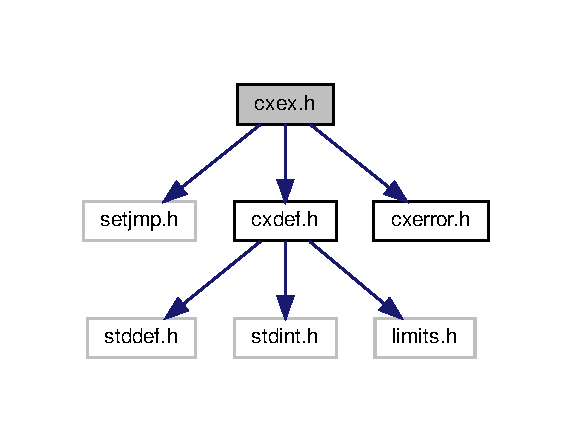
\includegraphics[width=275pt]{a00012}
\end{center}
\end{figure}
This graph shows which files directly or indirectly include this file\+:
\nopagebreak
\begin{figure}[H]
\begin{center}
\leavevmode
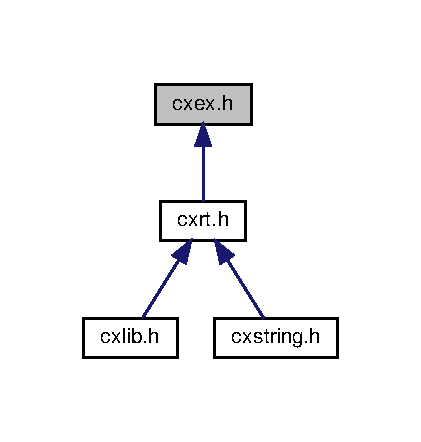
\includegraphics[width=202pt]{a00013}
\end{center}
\end{figure}
\subsection*{Classes}
\begin{DoxyCompactItemize}
\item 
struct \hyperlink{a00048}{cxexception}
\end{DoxyCompactItemize}
\subsection*{Macros}
\begin{DoxyCompactItemize}
\item 
\mbox{\Hypertarget{a00011_a099d212cb0554607ddc5f97f459108f8}\label{a00011_a099d212cb0554607ddc5f97f459108f8}} 
\#define {\bfseries C\+X\+E\+X\+\_\+\+V\+E\+R\+S\+I\+ON}~1000000L
\item 
\mbox{\Hypertarget{a00011_a07394dfadb1e836bb044fd133a0b5fdc}\label{a00011_a07394dfadb1e836bb044fd133a0b5fdc}} 
\#define {\bfseries cxtry}~if(!cxex\+\_\+setjmp($\ast$C\+X\+E\+X\+\_\+\+T\+RY())) \{
\item 
\mbox{\Hypertarget{a00011_a5d2ea9622f3bd15d8e8489663e04b11b}\label{a00011_a5d2ea9622f3bd15d8e8489663e04b11b}} 
\#define {\bfseries cxcatch}(...)~C\+X\+E\+X\+\_\+\+E\+N\+D\+\_\+\+T\+RY(); \} else if(C\+X\+E\+X\+\_\+\+C\+A\+T\+CH(0, \#\#\+\_\+\+\_\+\+V\+A\+\_\+\+A\+R\+G\+S\+\_\+\+\_\+, (\hyperlink{a00048}{cxexception\+\_\+t})\{\}))
\item 
\mbox{\Hypertarget{a00011_a6eb910a21c7df5cfaef2b0283101205d}\label{a00011_a6eb910a21c7df5cfaef2b0283101205d}} 
\#define {\bfseries cxthrow\+\_\+ret}(ex,  ret)~cxex\+\_\+longjmp($\ast$C\+X\+E\+X\+\_\+\+T\+H\+R\+OW(ex, ret), 1)
\item 
\mbox{\Hypertarget{a00011_a868460d46c56b694c6aa3f18464c9c4d}\label{a00011_a868460d46c56b694c6aa3f18464c9c4d}} 
\#define {\bfseries cxthrow}(ex)~cxthrow\+\_\+ret(ex, 0)
\item 
\mbox{\Hypertarget{a00011_aaac72ecb8338617ac54c2e50334d92ef}\label{a00011_aaac72ecb8338617ac54c2e50334d92ef}} 
\#define {\bfseries cxex\+\_\+setjmp}(jump)~sigsetjmp(jump, 1)
\item 
\mbox{\Hypertarget{a00011_a4ec477263777d3fa887e5451b3ec14f5}\label{a00011_a4ec477263777d3fa887e5451b3ec14f5}} 
\#define {\bfseries cxex\+\_\+longjmp}~siglongjmp
\end{DoxyCompactItemize}
\subsection*{Typedefs}
\begin{DoxyCompactItemize}
\item 
\mbox{\Hypertarget{a00011_a6a643c4c3fe776c4e158afba6ac87c7a}\label{a00011_a6a643c4c3fe776c4e158afba6ac87c7a}} 
typedef struct \hyperlink{a00048}{cxexception} {\bfseries cxexception\+\_\+t}
\end{DoxyCompactItemize}
\subsection*{Functions}
\begin{DoxyCompactItemize}
\item 
\mbox{\Hypertarget{a00011_a12358a045dfda6e1f68e043ee6fd0f4b}\label{a00011_a12358a045dfda6e1f68e043ee6fd0f4b}} 
int {\bfseries cxex\+\_\+istype} (\hyperlink{a00048}{cxexception\+\_\+t} except, \hyperlink{a00048}{cxexception\+\_\+t} other)
\end{DoxyCompactItemize}
\subsection*{Variables}
\begin{DoxyCompactItemize}
\item 
\mbox{\Hypertarget{a00011_afd15a1d98ac79a209f475756608bf619}\label{a00011_afd15a1d98ac79a209f475756608bf619}} 
cxdef\+\_\+thread\+\_\+local \hyperlink{a00048}{cxexception\+\_\+t} {\bfseries cxexcept}
\item 
\mbox{\Hypertarget{a00011_ac73de8289fd5bc03032a3725c501dca1}\label{a00011_ac73de8289fd5bc03032a3725c501dca1}} 
\hyperlink{a00048}{cxexception\+\_\+t} {\bfseries C\+X\+Exception}
\end{DoxyCompactItemize}


\subsection{Detailed Description}
Exception handling. 


\hypertarget{a00014}{}\section{cxlib.\+h File Reference}
\label{a00014}\index{cxlib.\+h@{cxlib.\+h}}


Single header file for entire library.  


{\ttfamily \#include $<$cxrt.\+h$>$}\newline
Include dependency graph for cxlib.\+h\+:
% FIG 0
\subsection*{Macros}
\begin{DoxyCompactItemize}
\item 
\mbox{\Hypertarget{a00014_a85ec71647670ef7260303289e48029fb}\label{a00014_a85ec71647670ef7260303289e48029fb}} 
\#define {\bfseries C\+X\+L\+I\+B\+\_\+\+V\+E\+R\+S\+I\+ON}~1000000L
\end{DoxyCompactItemize}


\subsection{Detailed Description}
Single header file for entire library. 


\hypertarget{a00017}{}\section{cxmem.\+h File Reference}
\label{a00017}\index{cxmem.\+h@{cxmem.\+h}}


Memory management.  


{\ttfamily \#include $<$stdlib.\+h$>$}\newline
{\ttfamily \#include $<$cxerror.\+h$>$}\newline
{\ttfamily \#include $<$cxui.\+h$>$}\newline
{\ttfamily \#include $<$cxdef.\+h$>$}\newline
{\ttfamily \#include $<$cxrt\+\_\+mutex.\+h$>$}\newline
Include dependency graph for cxmem.\+h\+:
\nopagebreak
\begin{figure}[H]
\begin{center}
\leavevmode
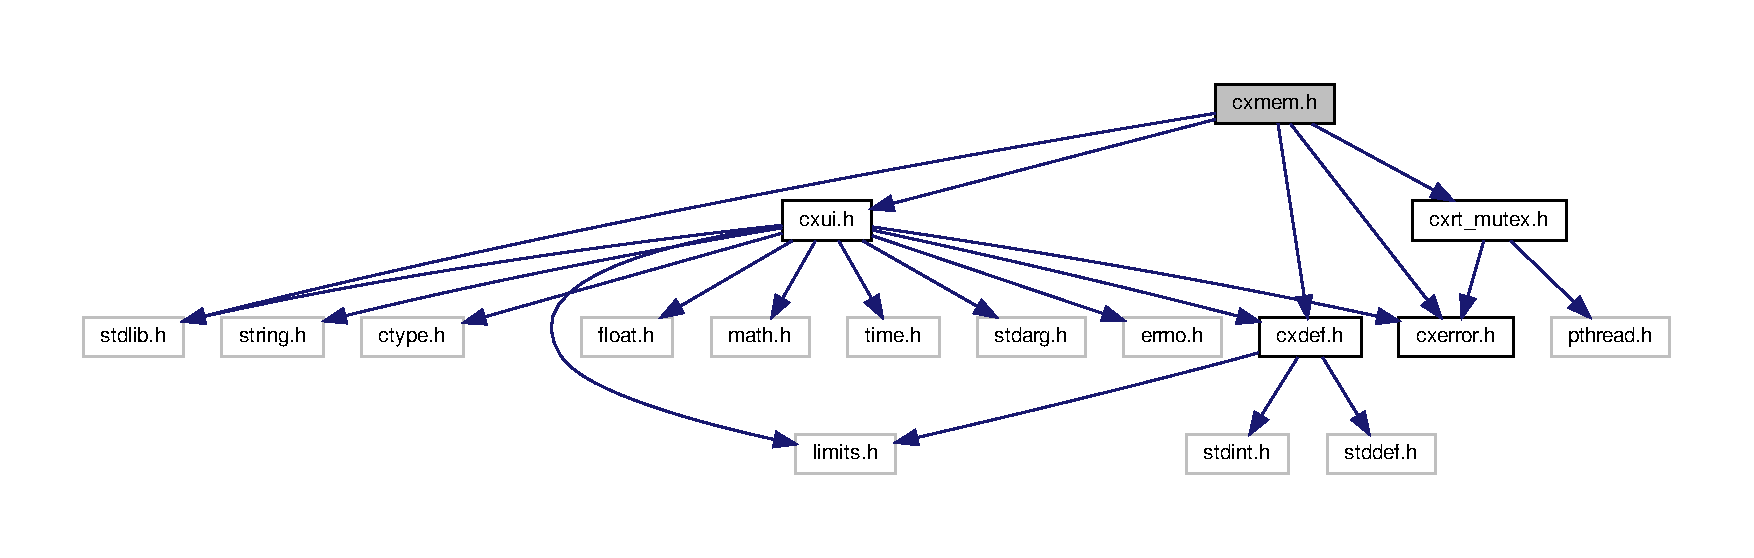
\includegraphics[width=350pt]{a00018}
\end{center}
\end{figure}
This graph shows which files directly or indirectly include this file\+:
\nopagebreak
\begin{figure}[H]
\begin{center}
\leavevmode
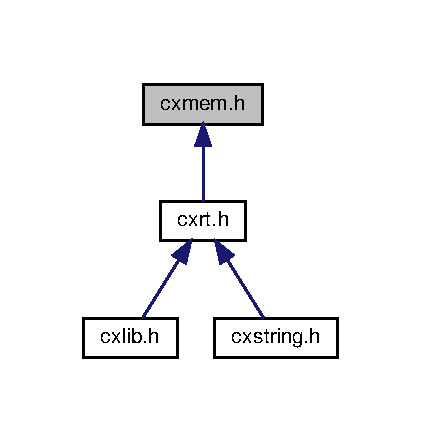
\includegraphics[width=202pt]{a00019}
\end{center}
\end{figure}
\subsection*{Classes}
\begin{DoxyCompactItemize}
\item 
struct \hyperlink{a00056}{cxmem\+\_\+storage}
\end{DoxyCompactItemize}
\subsection*{Macros}
\begin{DoxyCompactItemize}
\item 
\mbox{\Hypertarget{a00017_a71a23f5cbe64e9b426aabef1e04485a1}\label{a00017_a71a23f5cbe64e9b426aabef1e04485a1}} 
\#define {\bfseries C\+X\+M\+E\+M\+\_\+\+V\+E\+R\+S\+I\+ON}~1000000L
\item 
\mbox{\Hypertarget{a00017_ab3c2fc6fb7e39deb7335561f528e0c0c}\label{a00017_ab3c2fc6fb7e39deb7335561f528e0c0c}} 
\#define {\bfseries C\+X\+M\+E\+M\+\_\+\+D\+E\+F\+A\+U\+L\+T\+\_\+\+S\+T\+O\+R\+A\+G\+E\+\_\+\+C\+AP}~8
\item 
\mbox{\Hypertarget{a00017_a5707b6d44fd77907d5f2acea86cb40bb}\label{a00017_a5707b6d44fd77907d5f2acea86cb40bb}} 
\#define {\bfseries cxstatic}~(\&C\+X\+M\+E\+M\+\_\+\+S\+T\+A\+T\+IC)
\item 
\mbox{\Hypertarget{a00017_a2ab107701ba86364a8b580c2ed01881f}\label{a00017_a2ab107701ba86364a8b580c2ed01881f}} 
\#define {\bfseries cxthread\+\_\+local}~(\&C\+X\+R\+U\+N\+T\+I\+M\+E.\+storage)
\end{DoxyCompactItemize}
\subsection*{Typedefs}
\begin{DoxyCompactItemize}
\item 
\mbox{\Hypertarget{a00017_aace66181c4f439c1f67b868f3e930ec1}\label{a00017_aace66181c4f439c1f67b868f3e930ec1}} 
typedef struct \hyperlink{a00056}{cxmem\+\_\+storage} {\bfseries cxmem\+\_\+storage\+\_\+t}
\end{DoxyCompactItemize}
\subsection*{Functions}
\begin{DoxyCompactItemize}
\item 
\mbox{\Hypertarget{a00017_a79f881f6b5d0e7240669c94efdd9a1fe}\label{a00017_a79f881f6b5d0e7240669c94efdd9a1fe}} 
cxaddress\+\_\+t {\bfseries cxmalloc} (\hyperlink{a00056}{cxmem\+\_\+storage\+\_\+t} $\ast$storage, cxsize\+\_\+t cap)
\item 
\mbox{\Hypertarget{a00017_ad0e71c095779be36c9f1b59bdb046ce3}\label{a00017_ad0e71c095779be36c9f1b59bdb046ce3}} 
cxaddress\+\_\+t {\bfseries cxrealloc} (cxaddress\+\_\+t addr, cxsize\+\_\+t cap)
\item 
\mbox{\Hypertarget{a00017_aa385ca512cff4b8c301e8a53433717ef}\label{a00017_aa385ca512cff4b8c301e8a53433717ef}} 
void {\bfseries cxfree} (cxaddress\+\_\+t addr)
\item 
\mbox{\Hypertarget{a00017_ad54d278ec209a424cadf8f9fadb12a16}\label{a00017_ad54d278ec209a424cadf8f9fadb12a16}} 
cxaddress\+\_\+t {\bfseries cxnew} (\hyperlink{a00056}{cxmem\+\_\+storage\+\_\+t} $\ast$storage, \hyperlink{a00076}{cxui\+\_\+t} $\ast$ui,...)
\item 
\mbox{\Hypertarget{a00017_a3db54ac7c72f2bc05eebe2d4a1af5ba1}\label{a00017_a3db54ac7c72f2bc05eebe2d4a1af5ba1}} 
void {\bfseries cxdelete} (cxaddress\+\_\+t addr)
\item 
\mbox{\Hypertarget{a00017_a82077f7f1f9c7357eab44f2723a5d4b0}\label{a00017_a82077f7f1f9c7357eab44f2723a5d4b0}} 
cxaddress\+\_\+t {\bfseries cxpush} (cxaddress\+\_\+t address)
\item 
\mbox{\Hypertarget{a00017_a88798e8e4491762a9ca0f5b7024a8d4d}\label{a00017_a88798e8e4491762a9ca0f5b7024a8d4d}} 
void {\bfseries cxpushall} ()
\item 
\mbox{\Hypertarget{a00017_abf00dae1b2b6acb3018f47db17101a3c}\label{a00017_abf00dae1b2b6acb3018f47db17101a3c}} 
cxaddress\+\_\+t {\bfseries cxrestore} (\hyperlink{a00056}{cxmem\+\_\+storage\+\_\+t} $\ast$storage, cxaddress\+\_\+t address)
\item 
\mbox{\Hypertarget{a00017_a00ca5fd486c44a30fd7632301e9a20b0}\label{a00017_a00ca5fd486c44a30fd7632301e9a20b0}} 
void {\bfseries cxrestoreall} (\hyperlink{a00056}{cxmem\+\_\+storage\+\_\+t} $\ast$new\+\_\+storage, \hyperlink{a00056}{cxmem\+\_\+storage\+\_\+t} $\ast$old\+\_\+storage)
\end{DoxyCompactItemize}
\subsection*{Variables}
\begin{DoxyCompactItemize}
\item 
\mbox{\Hypertarget{a00017_a7615933cf4e71b063bbd553a2aa11de2}\label{a00017_a7615933cf4e71b063bbd553a2aa11de2}} 
\hyperlink{a00056}{cxmem\+\_\+storage\+\_\+t} {\bfseries C\+X\+M\+E\+M\+\_\+\+S\+T\+A\+T\+IC}
\item 
\mbox{\Hypertarget{a00017_a6e340b69c4d8beb1239b069f21829db6}\label{a00017_a6e340b69c4d8beb1239b069f21829db6}} 
\hyperlink{a00048}{cxexception\+\_\+t} {\bfseries C\+X\+Exception\+\_\+\+Memory}
\item 
\mbox{\Hypertarget{a00017_aec270a4fea4eedbfc32521b662268983}\label{a00017_aec270a4fea4eedbfc32521b662268983}} 
\hyperlink{a00048}{cxexception\+\_\+t} {\bfseries C\+X\+Exception\+\_\+\+Memory\+\_\+\+No\+Memory}
\item 
\mbox{\Hypertarget{a00017_a062da6eb8e13def13e9519836f17c50a}\label{a00017_a062da6eb8e13def13e9519836f17c50a}} 
\hyperlink{a00048}{cxexception\+\_\+t} {\bfseries C\+X\+Exception\+\_\+\+Memory\+\_\+\+Invalid\+Address}
\item 
\mbox{\Hypertarget{a00017_ac4706b050a8612db9e7c45ed2eceff0f}\label{a00017_ac4706b050a8612db9e7c45ed2eceff0f}} 
\hyperlink{a00048}{cxexception\+\_\+t} {\bfseries C\+X\+Exception\+\_\+\+Memory\+\_\+\+Invalid\+Push}
\item 
\mbox{\Hypertarget{a00017_a7862241f43b7647161f4c69a60ed2a18}\label{a00017_a7862241f43b7647161f4c69a60ed2a18}} 
\hyperlink{a00048}{cxexception\+\_\+t} {\bfseries C\+X\+Exception\+\_\+\+Memory\+\_\+\+Invalid\+Arg}
\end{DoxyCompactItemize}


\subsection{Detailed Description}
Memory management. 


\hypertarget{a00026}{}\section{cxstring.\+h File Reference}
\label{a00026}\index{cxstring.\+h@{cxstring.\+h}}


Strings.  


{\ttfamily \#include $<$string.\+h$>$}\newline
{\ttfamily \#include $<$ctype.\+h$>$}\newline
{\ttfamily \#include $<$cxrt.\+h$>$}\newline
Include dependency graph for cxstring.\+h\+:
% FIG 0
\subsection*{Classes}
\begin{DoxyCompactItemize}
\item 
struct \hyperlink{a00072}{cxstring}
\end{DoxyCompactItemize}
\subsection*{Macros}
\begin{DoxyCompactItemize}
\item 
\mbox{\Hypertarget{a00026_aeac35aa4fb83ef3b146347bb6385a5b0}\label{a00026_aeac35aa4fb83ef3b146347bb6385a5b0}} 
\#define {\bfseries C\+X\+S\+T\+R\+I\+N\+G\+\_\+\+V\+E\+R\+S\+I\+ON}~1000000L
\item 
\mbox{\Hypertarget{a00026_ac7d228210f438fd32024f6de3cc0eb77}\label{a00026_ac7d228210f438fd32024f6de3cc0eb77}} 
\#define {\bfseries C\+X\+S\+T\+R\+I\+N\+G\+\_\+\+D\+E\+F\+A\+U\+L\+T\+\_\+\+C\+AP}~8
\item 
\mbox{\Hypertarget{a00026_aed724d66437ae2f709d39f44e68ef873}\label{a00026_aed724d66437ae2f709d39f44e68ef873}} 
\#define {\bfseries cxstring\+\_\+includes}~cxstring\+\_\+contains
\item 
\mbox{\Hypertarget{a00026_aafb26af310693775a68bdcca40b83966}\label{a00026_aafb26af310693775a68bdcca40b83966}} 
\#define {\bfseries cxstring\+\_\+remove}~cxstring\+\_\+erase
\item 
\mbox{\Hypertarget{a00026_a878e400c242403fc5a2b736e3a1ece69}\label{a00026_a878e400c242403fc5a2b736e3a1ece69}} 
\#define {\bfseries cxstring\+\_\+search}~cxstring\+\_\+find
\item 
\mbox{\Hypertarget{a00026_aa1456f39cf8b871d043bc10bad1e2e7d}\label{a00026_aa1456f39cf8b871d043bc10bad1e2e7d}} 
\#define {\bfseries cxstring\+\_\+append}~cxstring\+\_\+concat
\item 
\mbox{\Hypertarget{a00026_a317d7942f1fd71079f6a6dc11ef6231d}\label{a00026_a317d7942f1fd71079f6a6dc11ef6231d}} 
\#define {\bfseries cxstring\+\_\+is\+\_\+empty}~cxstring\+\_\+empty
\item 
\mbox{\Hypertarget{a00026_afa17d12300611e8985407ea47070df94}\label{a00026_afa17d12300611e8985407ea47070df94}} 
\#define {\bfseries cxstring\+\_\+substr}~cxstring\+\_\+sub
\item 
\mbox{\Hypertarget{a00026_a40d13693bc5add409b6b13601b4fc102}\label{a00026_a40d13693bc5add409b6b13601b4fc102}} 
\#define {\bfseries cxstring\+\_\+substring}~cxstring\+\_\+sub
\item 
\mbox{\Hypertarget{a00026_a173c568ed7201c70ca8c487058d762e2}\label{a00026_a173c568ed7201c70ca8c487058d762e2}} 
\#define {\bfseries cxstr}(data)~\hyperlink{a00072}{cxstring}(data)
\end{DoxyCompactItemize}
\subsection*{Typedefs}
\begin{DoxyCompactItemize}
\item 
\mbox{\Hypertarget{a00026_a7c8cb74c1394a3e8b16552d9ca2d2e22}\label{a00026_a7c8cb74c1394a3e8b16552d9ca2d2e22}} 
typedef struct \hyperlink{a00072}{cxstring} {\bfseries cxstring\+\_\+t}
\end{DoxyCompactItemize}
\subsection*{Functions}
\begin{DoxyCompactItemize}
\item 
\mbox{\Hypertarget{a00026_aaf0291b3f4784ea60a958af062950e6b}\label{a00026_aaf0291b3f4784ea60a958af062950e6b}} 
\hyperlink{a00072}{cxstring\+\_\+t} {\bfseries cxstring\+\_\+construct} (\hyperlink{a00056}{cxmem\+\_\+storage\+\_\+t} $\ast$storage, char $\ast$data, cxsize\+\_\+t cap)
\item 
\mbox{\Hypertarget{a00026_aba7437afb6d8f85f32d47c018716043e}\label{a00026_aba7437afb6d8f85f32d47c018716043e}} 
void {\bfseries cxstring\+\_\+destruct} (\hyperlink{a00072}{cxstring\+\_\+t} str)
\item 
\mbox{\Hypertarget{a00026_ade4838a89cc9e461f4b4bd6e3c6fbe93}\label{a00026_ade4838a89cc9e461f4b4bd6e3c6fbe93}} 
void {\bfseries cxstring\+\_\+verify} (\hyperlink{a00072}{cxstring\+\_\+t} $\ast$str)
\item 
\mbox{\Hypertarget{a00026_abb8c6b1fe4ae233af6c87658cf80dd30}\label{a00026_abb8c6b1fe4ae233af6c87658cf80dd30}} 
\hyperlink{a00072}{cxstring\+\_\+t} {\bfseries cxstring} (char $\ast$data)
\item 
\mbox{\Hypertarget{a00026_a5d6cd107391b8ee47c8c8ce0c69a8e23}\label{a00026_a5d6cd107391b8ee47c8c8ce0c69a8e23}} 
\hyperlink{a00072}{cxstring\+\_\+t} {\bfseries cxstring\+\_\+cap} (char $\ast$data, cxsize\+\_\+t cap)
\item 
\mbox{\Hypertarget{a00026_a6999a363dd1b66b6f9624f8d8db70a4a}\label{a00026_a6999a363dd1b66b6f9624f8d8db70a4a}} 
\hyperlink{a00072}{cxstring\+\_\+t} {\bfseries cxstring\+\_\+at} (\hyperlink{a00072}{cxstring\+\_\+t} str, cxsize\+\_\+t i)
\item 
\mbox{\Hypertarget{a00026_a2e16727bc4fc1def1ee115678e86291e}\label{a00026_a2e16727bc4fc1def1ee115678e86291e}} 
\hyperlink{a00072}{cxstring\+\_\+t} {\bfseries cxstring\+\_\+sub} (\hyperlink{a00072}{cxstring\+\_\+t} str, cxsize\+\_\+t i, cxsize\+\_\+t size)
\item 
\mbox{\Hypertarget{a00026_af47d5df170c3b7063fd201986ae19f8e}\label{a00026_af47d5df170c3b7063fd201986ae19f8e}} 
\hyperlink{a00072}{cxstring\+\_\+t} {\bfseries cxstring\+\_\+erase} (\hyperlink{a00072}{cxstring\+\_\+t} str, cxsize\+\_\+t size)
\item 
\mbox{\Hypertarget{a00026_a09a551e9c1462b544fd5fdee0643d97f}\label{a00026_a09a551e9c1462b544fd5fdee0643d97f}} 
cxsize\+\_\+t {\bfseries cxstring\+\_\+size} (\hyperlink{a00072}{cxstring\+\_\+t} str)
\item 
\mbox{\Hypertarget{a00026_a7343a3c594bfd8dad231453d7dd37aff}\label{a00026_a7343a3c594bfd8dad231453d7dd37aff}} 
\hyperlink{a00072}{cxstring\+\_\+t} {\bfseries cxstring\+\_\+resize} (\hyperlink{a00072}{cxstring\+\_\+t} $\ast$str, cxsize\+\_\+t size)
\item 
\mbox{\Hypertarget{a00026_a39baecb2e2cf07742bb2b3dadf4990d0}\label{a00026_a39baecb2e2cf07742bb2b3dadf4990d0}} 
\hyperlink{a00072}{cxstring\+\_\+t} {\bfseries cxstring\+\_\+reserve} (\hyperlink{a00072}{cxstring\+\_\+t} $\ast$str, cxsize\+\_\+t cap)
\item 
\mbox{\Hypertarget{a00026_ab441e4a21aa272aa037d1ec140195178}\label{a00026_ab441e4a21aa272aa037d1ec140195178}} 
\hyperlink{a00072}{cxstring\+\_\+t} {\bfseries cxstring\+\_\+clear} (\hyperlink{a00072}{cxstring\+\_\+t} $\ast$str)
\item 
\mbox{\Hypertarget{a00026_a634c9663066f29ff9707b8e2d3da2729}\label{a00026_a634c9663066f29ff9707b8e2d3da2729}} 
\hyperlink{a00072}{cxstring\+\_\+t} {\bfseries cxstring\+\_\+copy} (\hyperlink{a00072}{cxstring\+\_\+t} des, \hyperlink{a00072}{cxstring\+\_\+t} src)
\item 
\mbox{\Hypertarget{a00026_aeb237db78af114958984c938dba4f98c}\label{a00026_aeb237db78af114958984c938dba4f98c}} 
\hyperlink{a00072}{cxstring\+\_\+t} {\bfseries cxstring\+\_\+insert} (\hyperlink{a00072}{cxstring\+\_\+t} des, cxsize\+\_\+t i, \hyperlink{a00072}{cxstring\+\_\+t} src)
\item 
\mbox{\Hypertarget{a00026_a39566cb811f44460e07107e8e99c1a33}\label{a00026_a39566cb811f44460e07107e8e99c1a33}} 
\hyperlink{a00072}{cxstring\+\_\+t} {\bfseries cxstring\+\_\+replace} (\hyperlink{a00072}{cxstring\+\_\+t} des, cxsize\+\_\+t size, \hyperlink{a00072}{cxstring\+\_\+t} src)
\item 
\mbox{\Hypertarget{a00026_ac12a5c56e702611eb7c6006f1b691a38}\label{a00026_ac12a5c56e702611eb7c6006f1b691a38}} 
\hyperlink{a00072}{cxstring\+\_\+t} {\bfseries cxstring\+\_\+concat} (\hyperlink{a00072}{cxstring\+\_\+t} des, \hyperlink{a00072}{cxstring\+\_\+t} src)
\item 
\mbox{\Hypertarget{a00026_aefa55d1bdf26f9672a87a004a4536ff8}\label{a00026_aefa55d1bdf26f9672a87a004a4536ff8}} 
\hyperlink{a00072}{cxstring\+\_\+t} {\bfseries cxstring\+\_\+swap} (\hyperlink{a00072}{cxstring\+\_\+t} $\ast$str1, \hyperlink{a00072}{cxstring\+\_\+t} $\ast$str2)
\item 
\mbox{\Hypertarget{a00026_ae82b55379c5523b993f2cd0dc35d8aac}\label{a00026_ae82b55379c5523b993f2cd0dc35d8aac}} 
\hyperlink{a00072}{cxstring\+\_\+t} {\bfseries cxstring\+\_\+clone} (\hyperlink{a00072}{cxstring\+\_\+t} str)
\item 
\mbox{\Hypertarget{a00026_af879ce4f5ad5c766d6e85e7091b535c0}\label{a00026_af879ce4f5ad5c766d6e85e7091b535c0}} 
int {\bfseries cxstring\+\_\+empty} (\hyperlink{a00072}{cxstring\+\_\+t} str)
\item 
\mbox{\Hypertarget{a00026_a9ab6eca9b23e57aaeb9497bad9f0e780}\label{a00026_a9ab6eca9b23e57aaeb9497bad9f0e780}} 
int {\bfseries cxstring\+\_\+compare} (\hyperlink{a00072}{cxstring\+\_\+t} str1, \hyperlink{a00072}{cxstring\+\_\+t} str2, int case\+\_\+sensitive)
\item 
\mbox{\Hypertarget{a00026_a04b30db16aa250d2693bb2a240c1df6b}\label{a00026_a04b30db16aa250d2693bb2a240c1df6b}} 
int {\bfseries cxstring\+\_\+equals} (\hyperlink{a00072}{cxstring\+\_\+t} str1, \hyperlink{a00072}{cxstring\+\_\+t} str2, int case\+\_\+sensitive)
\item 
\mbox{\Hypertarget{a00026_aa5a66d6c99bbb3d8305334c5a694f096}\label{a00026_aa5a66d6c99bbb3d8305334c5a694f096}} 
int {\bfseries cxstring\+\_\+starts\+\_\+with} (\hyperlink{a00072}{cxstring\+\_\+t} str1, \hyperlink{a00072}{cxstring\+\_\+t} str2, int case\+\_\+sensitive)
\item 
\mbox{\Hypertarget{a00026_aeab236e5406de3a806354d555ac3b9a6}\label{a00026_aeab236e5406de3a806354d555ac3b9a6}} 
int {\bfseries cxstring\+\_\+ends\+\_\+with} (\hyperlink{a00072}{cxstring\+\_\+t} str1, \hyperlink{a00072}{cxstring\+\_\+t} str2, int case\+\_\+sensitive)
\item 
\mbox{\Hypertarget{a00026_ac570d3c2e46b7fd8b110f26afd9ba306}\label{a00026_ac570d3c2e46b7fd8b110f26afd9ba306}} 
int {\bfseries cxstring\+\_\+contains} (\hyperlink{a00072}{cxstring\+\_\+t} str1, \hyperlink{a00072}{cxstring\+\_\+t} str2, int case\+\_\+sensitive)
\item 
\mbox{\Hypertarget{a00026_ab5102cb0231f838e4d55e7dd0e21cdd9}\label{a00026_ab5102cb0231f838e4d55e7dd0e21cdd9}} 
cxsize\+\_\+t {\bfseries cxstring\+\_\+find} (\hyperlink{a00072}{cxstring\+\_\+t} str1, \hyperlink{a00072}{cxstring\+\_\+t} str2, int case\+\_\+sensitive)
\item 
\mbox{\Hypertarget{a00026_aa8ec55f4db6bac0c10db887d97688d61}\label{a00026_aa8ec55f4db6bac0c10db887d97688d61}} 
cxsize\+\_\+t {\bfseries cxstring\+\_\+span} (\hyperlink{a00072}{cxstring\+\_\+t} str1, \hyperlink{a00072}{cxstring\+\_\+t} str2, int case\+\_\+sensitive)
\item 
\mbox{\Hypertarget{a00026_a13c33626c74c9bc0ab4cd08058b19f1f}\label{a00026_a13c33626c74c9bc0ab4cd08058b19f1f}} 
\hyperlink{a00072}{cxstring\+\_\+t} {\bfseries cxstring\+\_\+trim} (\hyperlink{a00072}{cxstring\+\_\+t} str)
\item 
\mbox{\Hypertarget{a00026_ac1b5285b5a64bfd1974b906bf00b04f9}\label{a00026_ac1b5285b5a64bfd1974b906bf00b04f9}} 
\hyperlink{a00072}{cxstring\+\_\+t} {\bfseries cxstring\+\_\+strip} (\hyperlink{a00072}{cxstring\+\_\+t} str)
\item 
\mbox{\Hypertarget{a00026_a05d7cb78f4e113701f7ebff39643375d}\label{a00026_a05d7cb78f4e113701f7ebff39643375d}} 
\hyperlink{a00072}{cxstring\+\_\+t} {\bfseries cxstring\+\_\+to\+\_\+lower} (\hyperlink{a00072}{cxstring\+\_\+t} str)
\item 
\mbox{\Hypertarget{a00026_aabaffed8700bf2131926aa76ed1c6cdd}\label{a00026_aabaffed8700bf2131926aa76ed1c6cdd}} 
\hyperlink{a00072}{cxstring\+\_\+t} {\bfseries cxstring\+\_\+to\+\_\+upper} (\hyperlink{a00072}{cxstring\+\_\+t} str)
\item 
\mbox{\Hypertarget{a00026_a4663bed5e303176831f983df6667d76f}\label{a00026_a4663bed5e303176831f983df6667d76f}} 
\hyperlink{a00072}{cxstring\+\_\+t} {\bfseries cxstring\+\_\+vprintf} (\hyperlink{a00072}{cxstring\+\_\+t} string, char $\ast$format, va\+\_\+list argv)
\item 
\mbox{\Hypertarget{a00026_a7759b8e61f6a384ce0981813a939bbd4}\label{a00026_a7759b8e61f6a384ce0981813a939bbd4}} 
int {\bfseries cxstring\+\_\+vscanf} (\hyperlink{a00072}{cxstring\+\_\+t} string, char $\ast$format, va\+\_\+list argv)
\item 
\mbox{\Hypertarget{a00026_a8099e18ca92bf5534cb2142aa2c4cdb9}\label{a00026_a8099e18ca92bf5534cb2142aa2c4cdb9}} 
\hyperlink{a00072}{cxstring\+\_\+t} {\bfseries cxstring\+\_\+printf} (\hyperlink{a00072}{cxstring\+\_\+t} string, char $\ast$format,...)
\item 
\mbox{\Hypertarget{a00026_a522ebdda1052895d963693f5ed156f71}\label{a00026_a522ebdda1052895d963693f5ed156f71}} 
int {\bfseries cxstring\+\_\+scanf} (\hyperlink{a00072}{cxstring\+\_\+t} string, char $\ast$format,...)
\end{DoxyCompactItemize}
\subsection*{Variables}
\begin{DoxyCompactItemize}
\item 
\mbox{\Hypertarget{a00026_a643caff68e8ac61182eb782b4e8ffe19}\label{a00026_a643caff68e8ac61182eb782b4e8ffe19}} 
\hyperlink{a00048}{cxexception\+\_\+t} {\bfseries C\+X\+Exception\+\_\+\+String}
\item 
\mbox{\Hypertarget{a00026_af8b0da91153c365a6ea0521c60809d24}\label{a00026_af8b0da91153c365a6ea0521c60809d24}} 
\hyperlink{a00048}{cxexception\+\_\+t} {\bfseries C\+X\+Exception\+\_\+\+String\+\_\+\+Invalid\+Arg}
\item 
\mbox{\Hypertarget{a00026_a5a62e9abf565e296eaca7d996f9fdd0f}\label{a00026_a5a62e9abf565e296eaca7d996f9fdd0f}} 
\hyperlink{a00048}{cxexception\+\_\+t} {\bfseries C\+X\+Exception\+\_\+\+String\+\_\+\+Invalid\+Pointer}
\item 
\mbox{\Hypertarget{a00026_afd5773832287930848fd2d9c6a4b0861}\label{a00026_afd5773832287930848fd2d9c6a4b0861}} 
\hyperlink{a00048}{cxexception\+\_\+t} {\bfseries C\+X\+Exception\+\_\+\+String\+\_\+\+Invalid\+Index}
\item 
\mbox{\Hypertarget{a00026_a177f51ddbf4e14a2a601c1184e8375d7}\label{a00026_a177f51ddbf4e14a2a601c1184e8375d7}} 
\hyperlink{a00048}{cxexception\+\_\+t} {\bfseries C\+X\+Exception\+\_\+\+String\+\_\+\+Invalid\+Size}
\item 
\mbox{\Hypertarget{a00026_abdc7440bf9edc0d809a27902856bd312}\label{a00026_abdc7440bf9edc0d809a27902856bd312}} 
\hyperlink{a00048}{cxexception\+\_\+t} {\bfseries C\+X\+Exception\+\_\+\+String\+\_\+\+Invalid\+Cap}
\item 
\mbox{\Hypertarget{a00026_aa2c7dd02559c16c8e5c74416dbb6d1ac}\label{a00026_aa2c7dd02559c16c8e5c74416dbb6d1ac}} 
\hyperlink{a00048}{cxexception\+\_\+t} {\bfseries C\+X\+Exception\+\_\+\+String\+\_\+\+Missing\+Null}
\end{DoxyCompactItemize}


\subsection{Detailed Description}
Strings. 


\chapter{Example Documentation}
\hypertarget{a00078}{}\section{/home/tux/dev/cx/examples/exceptions.\+c}
Examples of exception handling.


\begin{DoxyCodeInclude}

\textcolor{preprocessor}{#include <\hyperlink{a00014}{cxlib.h}>}

\textcolor{keywordtype}{int} func();

\textcolor{keywordtype}{int} main()
\{
    \_\_cxmain\_\_

    cxtry
    \{
        \textcolor{comment}{//All CX exceptions are derived from CXException}
        cxthrow(CXException);
    \}
    cxcatch()
    \{
        \textcolor{comment}{//cxexcept is the excpetion caught above}
        printf(\textcolor{stringliteral}{"caught %s\(\backslash\)n"}, cxexcept.type);

        \textcolor{comment}{//continues}
    \}

    cxtry
    \{
        cxbyte\_t *p = NULL;

        cxbyte\_t b = *p;
    \}
    \textcolor{comment}{//Multiple exceptions can be caught including seg faults}
    cxcatch(CXException\_Signal\_SegFault, CXException\_Memory\_NoMemory)
    \{
        printf(\textcolor{stringliteral}{"caught %s\(\backslash\)n"}, cxexcept.type);
    \}

    cxtry
    \{
        func();
    \}
    cxcatch(CXException\_Memory\_NoMemory)
    \{
        printf(\textcolor{stringliteral}{"caught %s\(\backslash\)n"}, cxexcept.type);
    \}

    cxreturn 0;
\}

\textcolor{keywordtype}{int} func()
\{
    \textcolor{comment}{//Initialize function}
    \_\_cxfunc\_\_

    cxthrow(CXException\_Memory\_NoMemory);

    \textcolor{comment}{//Dont forget to use cxreturn not return}
    cxreturn 0;
\}
\end{DoxyCodeInclude}
 
\hypertarget{a00080}{}\section{/home/tux/dev/cx/examples/hello\+\_\+world.\+c}
A hello world example.


\begin{DoxyCodeInclude}

\textcolor{preprocessor}{#include <\hyperlink{a00014}{cxlib.h}>}

\textcolor{keywordtype}{int} main()
\{
    \textcolor{comment}{//Initialize the runtime}
    \_\_cxmain\_\_

    printf(\textcolor{stringliteral}{"Hello World!\(\backslash\)n"});

    \textcolor{comment}{//You must use cxreturn not return}
    cxreturn 0;
\}
\end{DoxyCodeInclude}
 
\hypertarget{a00082}{}\section{/home/tux/dev/cx/examples/memory.\+c}
Examples of memory management


\begin{DoxyCodeInclude}

\textcolor{preprocessor}{#include <\hyperlink{a00014}{cxlib.h}>}

cxbyte\_t* func();

\textcolor{keywordtype}{int} main()
\{
    \textcolor{comment}{//Initialize the runtime}
    \_\_cxmain\_\_

    \textcolor{comment}{//All memory stored in cxauto is deallocated on the next cxreturn}
    cxaddress\_t addr = cxmalloc(cxauto, 1000);

    \textcolor{comment}{//But memory can be moved to another storage after allocation.}
    \textcolor{comment}{//All memory stored in cxstatic is deallocated when the program exits}
    cxrestore(cxstatic, addr);

    \textcolor{comment}{//Note that addr may come from malloc or cxmalloc}
    cxfree(addr);

    printf(\textcolor{stringliteral}{"%p\(\backslash\)n"}, func());

    \textcolor{comment}{//You must use cxreturn not return}
    cxreturn 0;
\}

cxbyte\_t* func()
\{
    \_\_cxfunc\_\_

    \textcolor{comment}{//We can also return function local memory by pushing it before returning}
    cxbyte\_t* addr = cxpush(cxmalloc(cxauto, 1000));

    cxreturn addr;
\}
\end{DoxyCodeInclude}
 
%--- End generated contents ---

% Index
\backmatter
\newpage
\phantomsection
\clearemptydoublepage
\addcontentsline{toc}{chapter}{Index}
\printindex

\end{document}
